\section{TỈ SỐ LƯỢNG GIÁC CỦA GÓC NHỌN} % Tên bài
\subsection{TRỌNG TÂM KIẾN THỨC}
\subsubsection{ĐỊNH NGHĨA TỈ SỐ LƯỢNG GIÁC CỦA GÓC NHỌN}
\begin{tomtat}
	Cho góc nhọn $\alpha$. Lúc này ta xét $\triangle ABC$ vuông tại $A$ có $\widehat{ABC}=\alpha$, ta có
	\begin{itemize}	
		\item Tỉ số giữa cạnh đối và cạnh huyền được gọi là sin của góc $\alpha$, kí hiệu là $\sin\alpha$.
		\item Tỉ số giữa cạnh kề và cạnh huyền được gọi là côsin của góc $\alpha$, kí hiệu là $\cos\alpha$.
		\item Tỉ số giữa cạnh đối và cạnh kề được gọi là tang của góc $\alpha$, kí hiệu là $\tan\alpha$.
		\item Tỉ số giữa cạnh kề và cạnh đối được gọi là côtang của góc $\alpha$, kí hiệu là $\cot\alpha$.
	\end{itemize}
	\immini{
	Bốn tỉ số trên được gọi là các tỉ số lượng giác góc nhọn $\alpha$. Trong hình vẽ bên ta có
	\begin{multicols}{2}
		\begin{itemize}	
			\item $\sin\alpha = \sin{B} = \dfrac{AC}{BC}$;
			\item $\cos\alpha = \cos{B} = \dfrac{AB}{BC}$;
			\item $\tan\alpha = \tan{B} = \dfrac{AC}{AB}$;
			\item $\cot\alpha = \cot{B} = w2\dfrac{AB}{AC}$.
		\end{itemize}
	\end{multicols}
	}{
	\begin{tikzpicture}[scale=0.8, font=\footnotesize, line join=round, line cap=round, >=stealth]
		\path 
		(0,0) coordinate (B)
		(3,0) coordinate (A)
		(3,4) coordinate (C);
		\draw (0,0) node[left]{$B$}--(1.5,0) node[below]{cạnh kề}--(3,0) node[right]{$A$}--(3,4) node[above]{$C$}--(0,0);
		\draw (C)--(B)node[midway,sloped,above]{cạnh huyền};
		\draw (A)--(C)node[midway,sloped,below]{cạnh đối};
		\pic[draw, angle radius=3mm]{right angle=B--A--C};
		\pic[draw, angle radius=3mm]{angle=A--B--C};
		\draw (0.3,0.3) node[right]{$\alpha$};
	\end{tikzpicture}
	}
	\begin{luuy}
		Với góc nhọn $\alpha$ ($0<\alpha<90^\circ$), ta có
		\begin{multicols}{3}
			\begin{itemize}
				\item $0<\sin\alpha<1$;
				\item $0<\cos\alpha<1$;
				\item $\cot\alpha=\dfrac{1}{\tan\alpha}$.
			\end{itemize}
		\end{multicols}
	\end{luuy}
	Ta có bảng các tỉ số lượng giác của các góc nhọn đặc biệt (góc $30^\circ,45^\circ,60^\circ$).
	\begin{center}
        \renewcommand{\arraystretch}{1.7}
		\begin{tabular}{|c|c|c|c|c|}
			\hline
			$\alpha$ & $\sin\alpha$ & $\cos\alpha$ & $\tan\alpha$ & $\cot\alpha$\\
			\hline
			$30^\circ$&$\dfrac{1}{2}$&$\dfrac{\sqrt{3}}{2}$&$\dfrac{\sqrt{3}}{3}$&$\sqrt{3}$\\
			\hline
			$45^\circ$&$\dfrac{\sqrt{2}}{2}$&$\dfrac{\sqrt{2}}{2}$&$1$&$1$\\
			\hline
			$60^\circ$&$\dfrac{\sqrt{3}}{2}$&$\dfrac{1}{2}$&$\sqrt{3}$&$\dfrac{\sqrt{3}}{3}$\\
			\hline
		\end{tabular}
	\end{center}
\subsubsection{TỈ SỐ LƯỢNG GIÁC CỦA HAI GÓC PHỤ NHAU}
\begin{nx}
	Hai góc được gọi là phụ nhau nếu tổng của chúng bằng $90^\circ$.
\end{nx}
Khi đó tỉ số lượng giác của chúng có mối liên hệ như sau: sin góc này bằng côsin góc kia, tang góc này bằng côtang góc kia. Cụ thể, xét góc nhọn $\alpha$, khi đó ta có $\alpha$ và $90^\circ-\alpha$ là hai góc phụ nhau nên
\begin{multicols}{2}
	\begin{itemize}
		\item $\sin(90^\circ-\alpha)=\cos\alpha$;
		\item $\cos(90^\circ-\alpha)=\sin\alpha$;
		\item $\tan(90^\circ-\alpha)=\cot\alpha$;
		\item $\cot(90^\circ-\alpha)=\tan\alpha$.
	\end{itemize}
\end{multicols}
\end{tomtat}
\subsection{CÁC DẠNG BÀI TẬP}
\begin{dang}{Tính tỉ số lượng giác của góc nhọn trong tam giác vuông}
\end{dang}
\begin{vd}%[Dự án EX-9-Đề Cương Toán 9]%[Nguyễn Ngọc Huy Trường]%[9H1N1-1]
	\immini{
		Tính các tỉ số lượng giác của góc $\alpha$ trong tam giác $ABC$ ở hình vẽ bên.
	}{
		\begin{tikzpicture}[scale=1, font=\footnotesize, line join=round, line cap=round, >=stealth]
			\def\a{2};
			\path 
			(0:\a) coordinate (C)
			(180:\a) coordinate (B)
			(60:\a) coordinate (A)
			($(B)!0.5!(C)$) coordinate (D)
			;
			\path pic["\scriptsize$\alpha$", angle eccentricity=2,draw,angle radius=5mm]{angle= C--B--A};
			\path pic[draw,angle radius=2mm]{right angle= B--A--C};
			\draw 
			(A)--(B) node[midway,above, sloped] {$12$}
			--(C) node[midway, below, sloped] {$15$}--cycle node[midway,right] {$9$}
			;
			\foreach \t/\g in {A/90,B/180,C/0}{
				\draw[fill=black] (\t) circle (1pt) node[shift={(\g:3mm)}]{$\t$};
			}
		\end{tikzpicture}
	}
	\loigiai{ Xét tam giác $ABC$ vuông tại $A$ với $\widehat{B}=\alpha$, ta có
		\begin{multicols}{2}
			\begin{itemize}
				\item $\sin\alpha=\dfrac{AC}{BC}=\dfrac{9}{15}=\dfrac{3}{5}$;
				\item $\cos\alpha=\dfrac{AB}{BC}=\dfrac{12}{15}=\dfrac{4}{5}$;
				\item $\tan\alpha=\dfrac{AC}{AB}=\dfrac{9}{12}=\dfrac{3}{4}$;
				\item $\cot\alpha=\dfrac{AB}{AC}=\dfrac{12}{9}=\dfrac{4}{3}$.
			\end{itemize}
		\end{multicols}
	}
\end{vd}

\begin{vd}%[Dự án EX-9-Đề Cương Toán 9]%[Nguyễn Ngọc Huy Trường]%[9H1H1-1]
	\immini
	{Tính tỉ số lượng giác của góc $B$ trong hình bên.
	}
	{\begin{tikzpicture}[scale=1, font=\footnotesize, line join=round, line cap=round, >=stealth]
			\def\a{2};
			\path 
			(0:\a) coordinate (B)
			(180:\a) coordinate (C)
			(60:\a) coordinate (A)
			($(B)!0.5!(C)$) coordinate (D)
			;
			\path pic[angle eccentricity=2,draw,angle radius=3mm]{angle= A--B--C};
			\path pic[draw,angle radius=2mm]{right angle= C--A--B};
			\draw 
			(A)--(C) node[midway,above, sloped] {$12$}
			--(B) --cycle;
			\draw (A)--(B) node[midway,right] {$5$};
			\foreach \t/\g in {A/90,C/180,B/0}
			\draw[fill=black] (\t) circle (1pt) node[shift={(\g:3mm)}]{$\t$};
		\end{tikzpicture}
	}
	\loigiai{
		Ta có $BC^2 = AB^2 + AC^2 = 5^2 + 12^2 = 169$ suy ra $BC = 13$. \\
		Xét tam giác $ABC$ vuông tại $A$, ta có
		\begin{multicols}{2}
			\begin{itemize}
				\item $\sin B =\dfrac{AC}{BC}=\dfrac{12}{13}$;
				\item $\cos B =\dfrac{AB}{BC}=\dfrac{5}{13}$;
				\item $\tan B =\dfrac{AC}{AB}=\dfrac{12}{5}$;
				\item $\cot B =\dfrac{AB}{AC}=\dfrac{5}{12}$.
			\end{itemize}
		\end{multicols}
	}
\end{vd}

\begin{bt}%[Dự án EX-9-Đề Cương Toán 9]%[Nguyễn Ngọc Huy Trường]%%[9H1H1-1]
	Tính các tỉ số lượng giác của góc nhọn $A$ trong mỗi tam giác vuông $ABC$ có $\widehat{B}=90^\circ$ ở các hình sau.
	\begin{multicols}{4}
			\begin{enumerate}
				\item
				\begin{tikzpicture}[scale=1, font=\footnotesize, line join=round, line cap=round, >=stealth]
					\def\a{2.5};
					\path (0:0) coordinate (B)
					(0:\a) coordinate (C)
					(B)+(90:0.7*\a) coordinate (A)
					($(B)!0.5!(C)$) coordinate (D);
					\path pic[draw,angle radius=3mm]{right angle= A--B--C};
					\path pic[draw,angle radius=3mm]{angle= B--A--C};
					\draw (A)--(B) node[midway,left] {$3$}
					--(C) node[midway,below] {$4$}
					--cycle node[midway,right,yshift=3pt] {$5$}
					;
					\foreach \t/\g in {A/90,B/-90,C/-90}{
					\draw[fill=black] (\t) circle (1pt) node[shift={(\g:3mm)},font=\scriptsize]{$\t$};
					}
				\end{tikzpicture}
				\item 
				\begin{tikzpicture}[scale=1, font=\footnotesize, line join=round, line cap=round, >=stealth]
					\def\a{2};
					\path 
					(0:\a) coordinate (C)
					(180:\a) coordinate (B)
					(150:\a) coordinate (A)
					($(B)!0.5!(C)$) coordinate (D);
					\path pic[angle eccentricity=2,draw,angle radius=5mm]{angle= A--C--B};
					\path pic[draw,angle radius=3mm]{right angle= B--A--C};
					\draw 
					(A)--(B) node[midway,left] {$1$}
					--(C) node[midway, below] {$\sqrt{17}$}--cycle node[midway, above] {$4$}
					;
					\foreach \t/\g/\i in {A/90/B,B/-90/C,C/-90/A}{
						\draw[fill=black] (\t) circle (1pt) node[shift={(\g:3mm)}]{$ \i $};
					}
				\end{tikzpicture}
				\item 
				\begin{tikzpicture}[scale=1, font=\footnotesize, line join=round, line cap=round, >=stealth]
					\def\a{2.5};
					\path (0:0) coordinate (B)
					(0:\a) coordinate (C)
					(C)+(-90:0.85*\a) coordinate (A)
					(A)+(180:0.5*\a) coordinate (O);
					\path pic[draw,angle radius=3mm]{right angle= A--C--B};
					\path pic[draw,angle radius=3mm]{angle= C--A--B};
					\draw (A)--(B) node[midway,left,xshift=-3pt] {$3$}
					--(C) 
					--cycle node[midway,right,yshift=4pt] {$2$}
					;
					\foreach \t/\g/\i in {A/-90/A,B/90/C,C/90/B}{
						\draw[fill=black] (\t) circle (1pt) node[shift={(\g:3mm)}]{$ \i $};
					}
				\end{tikzpicture}
				\item 
				\begin{tikzpicture}[scale=1, font=\footnotesize, line join=round, line cap=round, >=stealth]
					\def\a{2.5};
					\path (0:0) coordinate (B)
					(180:\a) coordinate (C)
					(B)+(90:0.7*\a) coordinate (A)
					($(B)!0.5!(C)$) coordinate (D);
					\path pic[draw,angle radius=3mm]{right angle= A--B--C};
					\path pic[draw,angle radius=3mm]{angle= B--C--A};
					\draw (A)--(B) node[midway,right] {$\sqrt{6}$}
					--(C) node[midway,below] {$\sqrt{10}$}
					--cycle 
					;
					\foreach \t/\g/\i in {A/90/C,B/-90/B,C/-90/A}{
						\draw[fill=black] (\t) circle (1pt) node[shift={(\g:3mm)}]{$ \i $};
					}
				\end{tikzpicture}
			\end{enumerate}
			\end{multicols}
	\loigiai{
		\begin{enumerate}
			\item Ta có
			\begin{multicols}{2}
				\begin{itemize}
					\item $\sin A=\dfrac{BC}{AC}=\dfrac{4}{5};$\quad
					\item $\cos A=\dfrac{AB}{AC}=\dfrac{3}{5};$\quad
					\item $\tan A=\dfrac{BC}{AB}=\dfrac{4}{3};$\quad
					\item $\cot A=\dfrac{AB}{BC}=\dfrac{3}{4}.$
				\end{itemize}
			\end{multicols}
			\item Ta có
			\begin{multicols}{2}
				\begin{itemize}
					\item$\sin A=\dfrac{BC}{AC}=\dfrac{1}{\sqrt{17}};$\quad
					\item$\cos A=\dfrac{AB}{AC}=\dfrac{4}{\sqrt{17}};$\quad
					\item$\tan A=\dfrac{BC}{AB}=\dfrac{1}{4};$\quad
					\item$\cot A=\dfrac{AB}{BC}=\dfrac{4}{1}.$
				\end{itemize}
			\end{multicols}
			\item Xét $\triangle ABC$ vuông tại $B$, ta có	$BC=\sqrt{3^2-2^2}=\sqrt{5}$. Khi đó
			\begin{multicols}{2}
				\begin{itemize}
					\item$\sin A=\dfrac{BC}{AC}=\dfrac{\sqrt{5}}{3};$\quad
					\item$\cos A=\dfrac{AB}{AC}=\dfrac{2}{3};$\quad
					\item$\tan A=\dfrac{BC}{AB}=\dfrac{\sqrt{5}}{2};$\quad
					\item$\cot A=\dfrac{AB}{BC}=\dfrac{2}{\sqrt{5}}.$
				\end{itemize}
			\end{multicols}
			\item Xét $\triangle ABC$ vuông tại $B$, ta có $AC=\sqrt{\left(\sqrt{10}\right)^2-\left(\sqrt{6}\right)^2}=2$. Khi đó
			\begin{multicols}{2}
				\begin{itemize}
					\item $\sin A=\dfrac{BC}{AC}=\dfrac{\sqrt{6}}{2};$\quad
					\item$\cos A=\dfrac{AB}{AC}=\dfrac{\sqrt{10}}{2};$\quad
					\item$\tan A=\dfrac{BC}{AB}=\dfrac{\sqrt{6}}{\sqrt{10}};$\quad
					\item$\cot A=\dfrac{AB}{BC}=\dfrac{\sqrt{10}}{\sqrt{6}}.$
				\end{itemize}
			\end{multicols}
		\end{enumerate}
	}
\end{bt}

\begin{bt}%[Dự án EX-9-Đề Cương Toán 9]%[Nguyễn Ngọc Huy Trường]%[9H1H1-1]
	Cho tam giác $ABC$ vuông tại $A$. Tính các tỉ số lượng giác của góc $B$ trong mỗi trường hợp sau
	\begin{multicols}{2}
		\begin{enumerate}
			\item $BC=5$ cm; $AB=3$ cm;
			\item $BC=13$ cm; $AC=12$ cm;
			\item $BC=5\sqrt{2}$ cm; $AB=5$ cm;
			\item $AB=a\sqrt{3}$; $AC=a$.
		\end{enumerate}
	\end{multicols}
	\loigiai{
		\begin{enumerate}
			\item Áp dụng định lí Pythagore ta được $AC=\sqrt{5^2-3^2}=4$ cm. Tỉ số lượng giác của $\widehat{B}$ là
			\begin{multicols}{2}
				\begin{itemize}
					\item $\sin B=\dfrac{AC}{BC}=\dfrac{4}{5}$;\quad 
					\item$\cos B=\dfrac{AB}{BC}=\dfrac{3}{5}$;\quad 
					\item$\tan B=\dfrac{AC}{AB}=\dfrac{4}{3}$;\quad 
					\item$\cot B=\dfrac{AB}{AC}=\dfrac{3}{4}$.
				\end{itemize}
			\end{multicols}
			\item Áp dụng định lí Pythagore ta được $AB=\sqrt{13^2-12^2}=5$ cm. Tỉ số lượng giác của $\widehat{B}$ là
			\begin{multicols}{2}
				\begin{itemize}
					\item $\sin B=\dfrac{AC}{BC}=\dfrac{12}{13}$;\quad 
					\item$\cos B=\dfrac{AB}{BC}=\dfrac{5}{13}$;\quad 
					\item$\tan B=\dfrac{AC}{AB}=\dfrac{12}{5}$;\quad 
					\item$\cot B=\dfrac{AB}{AC}=\dfrac{5}{12}$.
				\end{itemize}
			\end{multicols}
			\item Áp dụng định lí Pythagore ta được $AC=\sqrt{\left(5\sqrt{2}\right)^2-5^2}=5$ cm. Ta có tam giác $ABC$ là tam giác vuông cân nên tỉ số lượng giác của $\widehat{B}$ là
			\begin{multicols}{2}
				\begin{itemize}
					\item $\sin B=\cos B=\dfrac{AB}{BC}=\dfrac{5}{5\sqrt{2}}
                     = \dfrac{\sqrt{2}}{2}$;\quad 
					\item $\tan B=\cot B=\dfrac{AB}{AC}=\dfrac{5}{5}=1$.
				\end{itemize}
			\end{multicols}
			\item Ta có $\cot B=\dfrac{AB}{AC}=\dfrac{a\sqrt{3}}{a}=\sqrt{3}$ nên $\widehat{B}=30^\circ$. Do đó
			\begin{itemize}
				\item $\sin B=\sin 30^\circ=\dfrac{1}{2}$;\quad 
				\item$\cos B=\cos 30^\circ=\dfrac{\sqrt{3}}{2}$;\quad 
				\item$\tan B=\tan 30^\circ=\dfrac{\sqrt{3}}{3}$.
			\end{itemize}
		\end{enumerate}
	}
\end{bt}

\begin{bt}%[Dự án EX-9-Đề Cương Toán 9]%[Nguyễn Ngọc Huy Trường]%[9H1H1-1]
	Cho tam giác $MNP$ có $MN=5$ cm, $MP=12$ cm, $NP=13$ cm. Chứng minh tam giác $MNP$ vuông tại $M$. Từ đó, tính các tỉ số lượng giác của góc $N$.
	\loigiai{
		\immini{
			Ta có $NP^2=169$ và $MN^2+MP^2=169$. Suy ra $NP^2=MN^2+MP^2$. \\
			Theo định lý Pythagore đảo, ta có tam giác $MNP$ vuông tại $M$. \\
			Xét tam giác $MNP$ vuông tại $M$, ta có
			\begin{multicols}{2}
				\begin{itemize}
					\item $\sin {N}=\dfrac{MP}{NP}=\dfrac{12}{13};$\quad 
					\item $\cos {N}=\dfrac{MN}{NP}=\dfrac{5}{13};$\quad
					\item $\tan {N}=\dfrac{MP}{MN}=\dfrac{12}{5};$\quad 
					\item $\cot {N}=\dfrac{NM}{MP}=\dfrac{5}{12}.$
				\end{itemize}
			\end{multicols}
		}{\begin{tikzpicture}[scale=0.8, font=\footnotesize, line join=round, line cap=round, >=stealth]
				\coordinate (N) at (-3,0);
				\coordinate (P) at (3,0);
				\coordinate (D) at ($(N) + (60:1)$);
				\coordinate (M) at ($(N)!(P)!(D)$);
				\draw (M)--(N)--(P)--cycle;
				\foreach \i/\g in {M/90,N/-90,P/-90}
				\draw[fill=black](\i) circle (1pt) ($(\i)+(\g:3mm)$) node[scale=1]{$\i$};
				\pic[angle eccentricity=2,draw, angle radius=2mm]{right angle= N--M--P};
				\pic[angle eccentricity=2,draw, angle radius=3mm]{angle= P--N--M};
		\end{tikzpicture}}
	}
\end{bt}

\begin{bt}%[Dự án EX-9-Đề Cương Toán 9]%[Nguyễn Ngọc Huy Trường][9H1H1-2]
	Tam giác $ABC$ vuông tại $A$, $AB = 1{,}5$; $BC = 3{,}5$. Tính tỉ số lượng giác của góc $C$ rồi suy ra các tỉ số lượng giác của góc $B$.
	\loigiai
	{\immini{Ta có $AC^2 = BC^2 - AB^2 = 3{,}5^2 - 1{,}5^2 = 10$ suy ra $AC = \sqrt{10}$. Do đó
			\begin{itemize}
				\item $\cos B =\sin C =\dfrac{AB}{BC}=\dfrac{1{,}5}{3{,}5} = \dfrac{3}{7}$;
				\item $\sin B =\cos C =\dfrac{AC}{BC}=\dfrac{\sqrt{10}}{3{,}5} = \dfrac{2\sqrt{10}}{7}$;
				\item $\cot B =\tan C =\dfrac{AB}{AC}=\dfrac{1{,}5}{\sqrt{10}} = \dfrac{3\sqrt{10}}{20}$;
				\item $\tan B =\cot C =\dfrac{AC}{AB}=\dfrac{\sqrt{10}}{1{,}5} = \dfrac{2\sqrt{10}}{3}$.
			\end{itemize}
		}
		{\begin{tikzpicture}[scale=1, font=\footnotesize, line join=round, line cap=round, >=stealth]
				\tikzset{every node/.style={scale=1}}
				\coordinate (A) at (0,0);
				\coordinate (B) at (0,3);
				\coordinate (C) at (5.5,0);
				\coordinate (m) at ($(A)!0.5!(B)$);
				\coordinate (n) at ($(B)!0.5!(C)$);
				\draw 
				(A)--(B)--(C)--(A) 
				;	
				\draw[fill=black] 
				(A) circle (1pt) node[below] {$A$}
				(B) circle (1pt) node[above] {$B$}
				(C) circle (1pt) node[below] {$C$}
				(m) node[left] {$1{,}5$ cm}
				(n) node[above] {$3{,}5$ cm}
				;
				\draw pic[draw=black,angle radius=3mm] {right angle = B--A--C};	
			\end{tikzpicture}
		}
	}
\end{bt}

\begin{bt}%[Dự án EX-9-Đề Cương Toán 9]%[Nguyễn Ngọc Huy Trường][9H1H1-2]
	Tam giác $ABC$ cân tại $A$, có $BC = 6$, đường cao $AH = 4$. Tính các tỉ số lượng giác của góc $B$. 
	\loigiai
	{\immini{
        Tam giác $ABC$ cân tại $A$ có $AH$ là đường cao nên $AH$ cũng là trung tuyến, hay $H$ là trung điểm của $BC$.\\
        Khi đó, $BH = \dfrac{6}{2} = 3$ và $AB = \sqrt{4^2 + 3^2} = 5$. Suy ra
			\begin{itemize}
				\item $\sin B =\dfrac{AH}{AB}=\dfrac{4}{5}= 0,8; $\quad
				\item $\cos B =\dfrac{BH}{AB}=\dfrac{3}{5}= 0,6;$ \quad
				\item $\tan B = \dfrac{AH}{AB} = \dfrac{4}{3}; $\quad
				\item $\cot B = \dfrac{BH}{AH} = \dfrac{3}{4} = 0,75.$
			\end{itemize}
		}
		{\begin{tikzpicture}[scale=1, font=\footnotesize, line join=round, line cap=round, >=stealth]
		\path (0,0) coordinate (B)
		(6,0) coordinate (C)
		($(B)!0.5!(C)$) coordinate (H)
		($(H)+(90:4)$) coordinate (A)
		;
		\draw (A)--(B)--(C)--cycle (A)--(H);
		\foreach \x/\g in {A/90,B/180,C/0,H/-90}
		\draw[fill=black] (\x) circle (1pt) node[shift=(\g:3mm)] {$\x$};
		\draw pic[draw=black,angle radius=5pt] {right angle = C--H--A};
		\end{tikzpicture}
		}
	}
\end{bt}

\begin{bt}%[Dự án EX-9-Đề Cương Toán 9]%[Nguyễn Ngọc Huy Trường]%[9H1H1-1]
	Tính $\tan C$ trong hình vẽ sau.
	\begin{center}
		\begin{tikzpicture}[scale=1, font=\footnotesize, line join=round, line cap=round, >=stealth]
			\tikzset{every node/.style={scale=1}}
			\coordinate (A) at (0,0);
			\coordinate (B) at (0,3);
			\coordinate (C) at (5.5,0);
			\coordinate (H) at ($(B)!(A)!(C)$);
			\coordinate (m) at ($(B)!0.5!(H)$);
			\coordinate (n) at ($(A)!0.5!(B)$);
			\draw 
			(A)--(B)--(C)--(A)--(H) 
			;	
			\draw[fill=black] 
			(A) circle (1pt) node[below] {$A$}
			(B) circle (1pt) node[above] {$B$}
			(C) circle (1pt) node[below] {$C$}
			(m) node[above] {$3$}
			(n) node[left] {$6$}
			(H) circle (1pt) node[above right] {$H$}
			;
			\draw pic[draw=black,angle radius=5pt] {right angle = B--A--C};
			\draw pic[draw=black,angle radius=5pt] {right angle = C--H--A};
		\end{tikzpicture}
	\end{center}
	\loigiai
	{
		Ta có $AH^2 = AB^2 - BH^2 = 6^2 - 3^2 = 27$ suy ra $AH = 3 \sqrt{3}$.\\
		Do đó $\tan C = \cot B = \dfrac{BH}{AH} = \dfrac{3}{3 \sqrt{3}} = \dfrac{1}{\sqrt{3}}$.
	}
\end{bt}

\begin{bt}%[Dự án EX-9-Đề Cương Toán 9]%[Nguyễn Ngọc Huy Trường]%[9H1H1-2]
	Tính $\sin M + \cos N $ trong hình vẽ sau.
	\begin{center}
		\begin{tikzpicture}[scale=1, font=\footnotesize, line join=round, line cap=round, >=stealth]
			\tikzset{every node/.style={scale=1}}
			\coordinate (O) at (0,0);
			\coordinate (M) at (0,3);
			\coordinate (N) at (5.5,0);
			\coordinate (H) at ($(M)!(O)!(N)$);
			\coordinate (m) at ($(M)!0.5!(H)$);
			\coordinate (n) at ($(N)!0.5!(H)$);
			\draw 
			(O)--(M)--(N)--(O)--(H) 
			;	
			\draw[fill=black] 
			(O) circle (1pt) node[below] {$O$}
			(M) circle (1pt) node[above] {$M$}
			(N) circle (1pt) node[below] {$N$}
			(m) node[above] {$1$}
			(n) node[above] {$3$}
			(H) circle (1pt) node[above right] {$H$}
			;
			\draw pic[draw=black,angle radius=3mm] {right angle = M--O--N};
			\draw pic[draw=black,angle radius=3mm] {right angle = N--H--O};
		\end{tikzpicture}
	\end{center}
	\loigiai
	{  
        Do $\Delta HOM$ và $\Delta MON$ là các tam giác vuông nên $\widehat{HOM} = 90^\circ - \widehat{NMO} = \widehat{MNO}$.\\
        Khi đó, $\Delta MHO \sim \Delta OHN$ (g$-$g). Suy ra $\dfrac{OH}{HN} = \dfrac{MH}{OH}$, hay $OH^2 = HM\cdot HN$.\\
		Tính được $OH^2 = HM \cdot HN = 1 \cdot 3 = 3. Suy ra OH = \sqrt{3}$ và $OM = \sqrt{1 + 3} = 2$.\\
		Do đó $\sin M = \dfrac{OH}{OM} = \dfrac{\sqrt{3}}{2}$.\\
		Mặt khác $\cos N = \sin M = \dfrac{\sqrt{3}}{2}$ nên $\sin M + \cos N = \sqrt{3}$.
	}
\end{bt}

\begin{bt}%[Dự án EX-9-Đề Cương Toán 9]%[Nguyễn Ngọc Huy Trường]%[9H1V1-1]
	Cho hình vẽ sau. Tính $\sin C$ và $\tan B$.
	\begin{center}
	\begin{tikzpicture}[scale=1, font=\footnotesize, line join=round, line cap=round, >=stealth]
		\tikzset{every node/.style={scale=1}}
		\coordinate (A) at (0,0);
		\coordinate (B) at (0,3);
		\coordinate (C) at (5.5,0);
		\coordinate (H) at ($(B)!(A)!(C)$);
		\coordinate (m) at ($(B)!0.5!(H)$);
		\coordinate (n) at ($(C)!0.5!(H)$);
		\draw 
		(A)--(B)--(C)--(A)--(H) 
		;	
		\draw[fill=black] 
		(A) circle (1pt) node[below] {$A$}
		(B) circle (1pt) node[above] {$B$}
		(C) circle (1pt) node[below] {$C$}
		(m) node[above] {$1$}
		(n) node[above] {$2$}
		(H) circle (1pt) node[above right] {$H$}
		;
		\draw pic[draw=black,angle radius=5pt] {right angle = B--A--C};
		\draw pic[draw=black,angle radius=5pt] {right angle = B--H--A};
	\end{tikzpicture}
	\end{center}
	\loigiai
	{  
        Xét $\Delta ABH$ và $\Delta ABC$, có $\widehat{AHB} = \widehat{BAC} = 90^\circ$ và $\widehat{B}$ là góc chung.\\
        Do đó $\Delta ABH \sim \Delta CBA$ (g$-$g). Suy ra $\dfrac{AB}{CB} = \dfrac{BH}{AB}$, hay $AB^2 = BH\cdot BC$.\\
        Ta có $AB^2 = BC\cdot BH = 3\cdot 1$ suy ra $AB = \sqrt{3}$.\\
		Tính được $AH = \sqrt{AB^2 - BH^2} = \sqrt{2}$.\\
		Do đó $\sin C = \dfrac{AB}{BC} = \dfrac{\sqrt{3}}{3}$ và $\tan B = \dfrac{AH}{BH} = \dfrac{\sqrt{2}}{1} = \sqrt{2}$.
	}
\end{bt}

\begin{bt}%[Dự án EX-9-Đề Cương Toán 9]%[Nguyễn Ngọc Huy Trường]%[9H1V1-1]
	Tính các góc của hình thoi có hai đường chéo dài $2\sqrt{3}$ và $2$.
	\loigiai{
		\immini{
			Giả sử hình thoi $ABCD$ có $AC=2\sqrt{3}$, $BD=2$.\\
			Gọi $O$ là giao điểm của $AC$ và $BD$. Khi đó ta có $AC\perp BD$ tại $O$ và $BO=OD=1$; $AO=OC=\sqrt{3}$.\\
			Tam giác $ABO$ vuông tại $O$ có:
			$\tan{OAB}=\dfrac{BO}{OA}=\dfrac{1}{\sqrt{3}}$\\
			Suy ra $\widehat{OAB}=30^\circ$.\\
            Ta có: $\widehat{ABO}=90^\circ-\widehat{OAB}=90^\circ-30^\circ=60^\circ$.\\
			Vậy $\widehat{ABC}= \widehat{ADC} = 2\cdot\widehat{ABO} = 120^\circ$ và $\widehat{BAD}=\widehat{BCD}= 2\cdot\widehat{BAO} = 60^\circ$.
        }{
			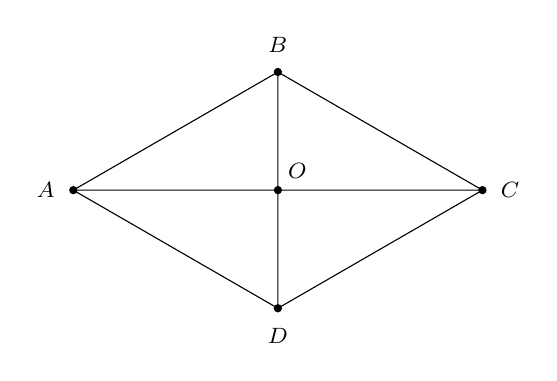
\begin{tikzpicture}[scale=1.5, font=\footnotesize, line join=round, line cap=round, >=stealth]
				\path (0,0) coordinate (A)
				({sqrt(3)},1) coordinate (B)
				({2*sqrt(3)},0) coordinate (C)
				({sqrt(3)},-1) coordinate (D)
				(intersection of A--C and B--D) coordinate (O)
				;
				\draw (A)--(B)--(C)--(D)--cycle (A)--(C) (B)--(D);
				\foreach\x/\y in {A/180,B/90,C/0,D/-90,O/45}{\fill (\x) circle (1pt) node[shift={(\y:0.35)}]{$\x$};}
			\end{tikzpicture}
		}
	}
\end{bt}

\begin{bt}%[Dự án EX-9-Đề Cương Toán 9]%[Nguyễn Ngọc Huy Trường]%[9H1H1-2]
	Cho tam giác $A B C$ vuông tại $A$, $AB=5$ cm, $AC=12$ cm.
	\begin{enumerate}
		\item Tính các tỉ số lượng giác của góc $B$.
		\item Từ kết quả trên suy ra các tỉ số lượng giác của góc $C$.
	\end{enumerate}
	\loigiai{
		\begin{enumerate}
			\item Áp dụng định lí Pythagore cho tam giác $A B C$ vuông tại $A$, ta có:
			\immini{
				$B C^{2}=A B^{2}+A C^{2}=5^{2}+12^{2}=169$, suy ra $BC=13$ cm. \\
				Khi đó
                \begin{multicols}{2}
                    \begin{itemize}
                        \item $\sin B=\dfrac{A C}{B C}=\dfrac{12}{13}$;
                        \item $\cos B=\dfrac{A B}{B C}=\dfrac{5}{13}$;
                        \item $\tan B=\dfrac{A C}{A B}=\dfrac{12}{5}$;
                        \item $\cot B=\dfrac{A B}{A C}=\dfrac{5}{12}$.
                    \end{itemize}
                \end{multicols}
                
				\item Do $\widehat{B}+\widehat{C}=90^{\circ}$ nên \\
                \begin{multicols}{2}
                    \begin{itemize}
                        \item $\sin C=\cos B=\dfrac{5}{13}$;
                        \item $\cos C=\sin B=\dfrac{12}{13}$;
                        \item $\tan C=\cot B=\dfrac{5}{12}$;
                        \item $\cot C=\tan B=\dfrac{12}{5}$.
                    \end{itemize}
                \end{multicols}
			}{
				\begin{tikzpicture}[scale=1, font=\footnotesize, line join=round, line cap=round, >=stealth]
					\tikzset{every node/.style={scale=1}}
					\coordinate (A) at (0,0);
					\coordinate (B) at (0,3);
					\coordinate (C) at (5.5,0);
					\coordinate (m) at ($(A)!0.5!(C)$);
					\coordinate (n) at ($(B)!0.5!(A)$);
					\draw 
					(A)--(B)--(C)--(A) 
					;	
					\draw[fill=black] 
					(A) circle (1pt) node[below] {$A$}
					(B) circle (1pt) node[above] {$B$}
					(C) circle (1pt) node[below] {$C$}
					(m) node[below] {$12$ cm}
					(n) node[right] {$5$ cm}
					;
					\draw pic[draw=black,angle radius=5pt] {right angle = B--A--C};	
				\end{tikzpicture}
			}
		\end{enumerate}
	}
\end{bt}

\begin{dang}{Tính giá trị biểu thức liên quan đến tỉ số lượng giác của một góc nhọn}
	\begin{enumerate}
		\item Sử dụng bảng tỉ số lượng giác của các góc nhọn đặc biệt (góc $30^\circ$, $45^\circ$, $60^\circ$).
		\item Sử dụng mối liên hệ về tỉ số lượng giác của hai góc phụ nhau.
	\end{enumerate}
\end{dang}

\begin{vd}%[Dự án EX-9-Đề Cương Toán 9]%[Nguyễn Ngọc Huy Trường]%[9H1N1-1]
	Tính giá trị của các biểu thức sau:
	\begin{multicols}{2}
		\begin{enumerate}
			\item $A=\sin45^\circ-\cos60^\circ$;
			\item $B=\sin^260^\circ-2\cos^260^\circ-\tan^260^\circ$;
			\item $C=\dfrac{1}{3}\cot^260^\circ+2\sin^230^\circ-\dfrac{3}{2}\cos^245^\circ$;
			\item $D=3\sin^245^\circ+2\cos^230^\circ+3\cot30^\circ$.
		\end{enumerate}
	\end{multicols}
	\loigiai{
		\begin{enumerate}
			\item $A = \sin 45^\circ - \cos 60^\circ = \dfrac{\sqrt{2}}{2} - \dfrac{1}{2} = \dfrac{\sqrt{2} - 1}{2}$.
			\item $B = \sin^2 60^\circ - 2\cos^2 60^\circ - \tan^2 60^\circ 
			= \left(\dfrac{\sqrt{3}}{2}\right)^2 - 2 \cdot\left(\dfrac{1}{2}\right)^2 - \left(\sqrt{3}\right)^2
			= \dfrac{3}{4} - \dfrac{2}{4} - 3 =  -\dfrac{11}{4}$.
			\item $C = \dfrac{1}{3}\cot ^2 60^\circ + 2\sin^2 30^\circ - \dfrac{3}{2} \cos^2 45^\circ 
			= \dfrac{1}{3} \cdot\left(\dfrac{1}{\sqrt{3}}\right)^2 + 2\cdot\left(\dfrac{1}{2}\right)^2 - \dfrac{3}{2}\cdot\left(\dfrac{\sqrt{2}}{2}\right)^2
			= \dfrac{1}{9} + \dfrac{1}{2} - \dfrac{3}{4} = \dfrac{-5}{36}$.
			\item $D = 3\sin^2 45^\circ + 2\cos^2 30^\circ + 3\cot 30^\circ 
			= 3\cdot\left(\dfrac{\sqrt{2}}{2}\right)^2 + 2\cdot\left(\dfrac{\sqrt{3}}{2} \right)^2 + 3\sqrt{3}
			= \dfrac{3}{2} + \dfrac{3}{2} + 3\sqrt{3} = 3 + 3\sqrt{3}$.
		\end{enumerate}
	}
\end{vd}

\begin{vd}%[Dự án EX-9-Đề Cương Toán 9]%[Nguyễn Ngọc Huy Trường]%[9H1H1-2]
	Tính giá trị của các biểu thức sau:
	\begin{multicols}{2}
		\begin{enumerate}
			\item $A=\sin23^\circ-\cos67^\circ$;
			\item $B=\tan18^\circ-\cot72^\circ$;
			\item $C=\sin10^\circ+\sin40^\circ-\cos50^\circ-\cos80^\circ$;
			\item $D=\sin25^\circ-\cos75^\circ+\dfrac{\cot25^\circ}{\tan75^\circ}$;
		\end{enumerate}
	\end{multicols}
	\loigiai{
		\begin{enumerate}
			\item $A = \sin 23^\circ - \cos 67^\circ = \sin 23^\circ - \sin 23^\circ = 0$.
			\item $B = \tan 18^\circ - \cot 72^\circ = \tan 18^\circ - \tan18^\circ=0$.
			\item $C = \sin 10^\circ + \sin 40^\circ - \cos 50^\circ - \cos 80^\circ=\sin 10^\circ + \sin 40^\circ-\sin 10^\circ - \sin 40^\circ=0$.
			\item $D = \sin 25^\circ - \cos 75^\circ + \dfrac{\cot 25^\circ}{\tan 75^\circ}=\sin25^\circ-\sin25^\circ+\dfrac{\cot25^\circ}{\cot25^\circ}=0+1=1$.
		\end{enumerate}
	}
\end{vd}

\begin{bt}%[Dự án EX-9-Đề Cương Toán 9]%[Nguyễn Ngọc Huy Trường]%[9H1H1-1]
	Tính giá trị của các biểu thức sau:
	\begin{multicols}{2}
		\begin{enumerate}
			\item $A=\sin^2 45^\circ+\cos ^2 45^\circ$;
			\item $B=\tan 30^\circ \cdot \cot 30^\circ$;
			\item $C=\dfrac{\sin 30^\circ\cdot\cos 60^\circ}{\tan 45^\circ}$;
			\item $D=\dfrac{2\cos 45^\circ}{\sqrt{2}}+\sqrt{3}\tan 30^\circ$;
			\item $E=\dfrac{2\sin 60^\circ}{\sqrt{3}}-\cot 45^\circ$;
			\item $F=\dfrac{2\sin 30^\circ - \sin 60^\circ}{\cos^230^\circ - \cos 60^\circ}$.
		\end{enumerate}
	\end{multicols}
	\loigiai{
		\begin{enumerate}
			\item $A=\sin^2 45^\circ+\cos^2 45^\circ=\left(\dfrac{\sqrt{2}}{2}\right)^2+\left(\dfrac{\sqrt{2}}{2}\right)^2=\dfrac{1}{2}+\dfrac{1}{2}=1$.
			\item $B=\tan 30^\circ \cdot \cot 30^\circ=\dfrac{\sqrt{3}}{3} \cdot \sqrt{3}=1$.
			\item $C=\dfrac{\sin 30^\circ\cdot\cos 60^\circ}{\tan 45^\circ}=\dfrac{\dfrac{1}{2}\cdot\dfrac{1}{2}}{1}=\dfrac{1}{4}$.
			\item $D=\dfrac{2\cos 45^\circ}{\sqrt{2}}+\sqrt{3}\tan 30^\circ=\dfrac{2\cdot\dfrac{\sqrt{2}}{2}}{\sqrt{2}}+\sqrt{3}\cdot \dfrac{\sqrt{3}}{3}=1+1=2$.
			\item $E=\dfrac{2\sin 60^\circ}{\sqrt{3}}-\cot 45^\circ=\dfrac{2\cdot\dfrac{\sqrt{3}}{2}}{\sqrt{3}}-1=1-1=0$.
			\item $F=\dfrac{2\sin 30^\circ - \sin 60^\circ}{\cos^230^\circ - \cos 60^\circ}
				= \dfrac{2\cdot\dfrac{1}{2} - \dfrac{\sqrt{3}}{2}}{\left(\dfrac{\sqrt{3}}{2}\right)^2 - \dfrac{1}{2}}=\dfrac{1 - \dfrac{\sqrt{3}}{2}}{\dfrac{3}{4} - \dfrac{1}{2}}= 4 - 2\sqrt{3}$.
		\end{enumerate}
	}
\end{bt}

\begin{bt}%[Dự án EX-9-Đề Cương Toán 9]%[Nguyễn Ngọc Huy Trường]%[9H1H1-1]
	Tính giá trị của các biểu thức sau:
	\begin{enumerate}
		\item $A=4-\sin^2 45^\circ+2\cos^2 60^\circ-3\cot^2 45^\circ$;
		\item $B=\tan 45^\circ\cdot \cos 30^\circ\cdot\cot30^\circ$;
		\item $C=\sin 15^\circ+\sin 75^\circ-\cos 15^\circ-\cos 75^\circ+\sin 30^\circ$.
	\end{enumerate}
	\loigiai{
		\begin{enumerate}
			\item $A=4-\sin^2 45^\circ+2\cos^2 60^\circ-3\cot^2 45^\circ=4-\left(\dfrac{\sqrt{2}}{2}\right)^2+2\cdot\left(\dfrac{1}{2}\right)^2-3\cdot 1^2=1$.
			\item $B=\tan 45^\circ\cdot \cos 30^\circ\cdot\cot30^\circ=1\cdot\dfrac{\sqrt{3}}{2}\cdot\sqrt{3}=\dfrac{3}{2}$.
			\item Ta có
			\allowdisplaybreaks
			\begin{eqnarray*}
			C&=&\sin 15^\circ+\sin 75^\circ-\cos 15^\circ-\cos 75^\circ+\sin 30^\circ\\
			&=&\cos75^\circ+\cos15^\circ-\cos 15^\circ - \cos 75^\circ+\sin 30^\circ\\
			&=&\sin30^\circ \\
			&=&\dfrac{1}{2}.
			\end{eqnarray*}
		\end{enumerate}
	}
\end{bt}

\begin{bt}%[Dự án EX-9-Đề Cương Toán 9]%[Nguyễn Ngọc Huy Trường]%[9H1H1-2]
	\begin{enumerate}
		\item Viết các tỉ số lượng giác sau thành tỉ số lượng giác của các góc nhỏ hơn $45^\circ$.
		\begin{multicols}{4}
			\begin{itemize}
				\item $\sin 55^\circ$;
				\item $\cos 62^\circ$;
				\item $\tan 57^\circ$;
				\item $\cot 64^\circ$.
			\end{itemize}
		\end{multicols}
		\item Tính $\dfrac{\tan25^\circ}{\cot 65^\circ}$, $\tan 34^\circ - \cot 56^\circ$.
	\end{enumerate}
	\loigiai{
		\begin{enumerate}
			\item
                \begin{itemize}
                    \item $\sin 55^\circ = \cos (90^\circ - 55^\circ) = \cos 35^\circ$;
                    \item $\cos 62^\circ = \sin (90^\circ - 62^\circ) = \sin 28^\circ$;
                    \item $\tan 57^\circ = \cot (90^\circ - 57^\circ) = \cot 33^\circ$;
                    \item $\cot 64^\circ = \tan (90^\circ - 64^\circ) = \tan 26^\circ$.
                \end{itemize}
			\item
                \begin{itemize}
                    \item $\dfrac{\tan 25^\circ}{\cot 65^\circ} = \dfrac{\cot (90^\circ - 25^\circ)}{\cot 65^\circ} = \dfrac{\cot 65^\circ}{\cot 65^\circ} = 1$;
                    \item $\tan 34^\circ - \cot 56^\circ = \tan 34^\circ - \tan (90^\circ - 56^\circ) = \tan 34^\circ - \tan 34^\circ = 0$.
                \end{itemize}
		\end{enumerate}
	}
\end{bt}

\begin{bt}%[Dự án EX-9-Đề Cương Toán 9]%[Nguyễn Ngọc Huy Trường]%[9H1N1-3]
	Không dùng máy tính hoặc bảng số, hãy tính giá trị của biểu thức $M = \sin^220^\circ + \cos^230^\circ - \sin^240^\circ - \sin^250^\circ + \cos^260^\circ + \sin^270^\circ$.
	\loigiai{
 		Ta có $\sin^270^\circ = \sin^2\left(90^\circ- 20^\circ\right) = \cos^220^\circ$.\\
 		Tương tự $\sin^250^\circ = \sin^2\left(90^\circ- 40^\circ\right) = \cos^240^\circ$ và $\cos^260^\circ = \cos^2\left(90^\circ- 30^\circ\right) = \sin^230^\circ$.\\
 		Do đó 
 		\allowdisplaybreaks
 		\begin{eqnarray*}
 			M &=& \sin^220^\circ + \cos^230^\circ - \sin^240^\circ - \cos^240^\circ + \sin^260^\circ + \cos^220^\circ\\
 			&=& \left(\sin^220^\circ + \cos^220^\circ\right) + \left(\cos^230^\circ + \sin^230^\circ\right) - \left(\sin^240^\circ + \cos^240^\circ\right) \\
			&=& 1 + 1 - 1 = 1.
 		\end{eqnarray*}
	}
\end{bt}

\begin{dang}{Sử dụng máy tính cầm tay để tính tỉ số lượng giác của một góc và tính góc}
\end{dang}
\begin{vd}%[Dự án EX-9-Đề Cương Toán 9]%[Nguyễn Ngọc Huy Trường]%[9H1N1-3]
	Sử dụng máy tính cầm tay tính các tỉ số lượng giác sau và làm tròn kết quả đến chữ số thập phân thứ ba:
	\begin{multicols}{2}
		\begin{enumerate}
			\item
			$\sin 27^\circ$, 
			$\cos 32^\circ 15'$, 
			$\tan 52^\circ 12'$ 
			và $\cot 35^\circ 23'$.
			\item
			$\sin 40^\circ 54'$,
			$\cos 52^\circ 15'$,
			$\tan 69^\circ 36'$
			và $\cot 25^\circ 18'$.
		\end{enumerate}
	\end{multicols}
	\loigiai{
		\begin{enumerate}
			\item
			\begin{tabular}{|l|l|l|}
				\hline
				Giá trị cần tính & Kết quả \\ \hline
				$\sin 27^\circ$ & $0{,}4539904997$ \\ \hline
				$\cos 32^\circ 15'$ & $0{,}8457278217$ \\ \hline
				$\tan 52^\circ 12'$ & $1{,}289192232$ \\ \hline
				$\cot 35^\circ 23'$ & $1{,}408003909$ \\ \hline
			\end{tabular} \\
			Làm tròn đến chữ số thập phân thứ ba ta được
            \begin{multicols}{2}
                \begin{itemize}
                    \item $\sin 27^\circ \approx 0{,}454$;
                    \item $\cos 32^\circ 15'\approx 0{,}846$;
                    \item $\tan 52^\circ 12' \approx 1{,}289$;
                    \item $\cot 35^\circ 23' \approx 1{,}408$.
                \end{itemize}
            \end{multicols}
			Lưu ý, $\cot 35^\circ 23' = \dfrac{1}{\tan 35^\circ 23'}$.
			\item
			\begin{tabular}{|l|l|l|}
				\hline
				Giá trị cần tính & Kết quả \\ \hline
				$\sin 40^\circ 54'$ & $0{,}6547408137$ \\ \hline
				$\cos 52^\circ 15'$ & $0{,}61221728$ \\ \hline
				$\tan 69^\circ 36'$ & $2{,}688918967$ \\ \hline
				$\cot 25^\circ 18'$ & $2{,}115516356$ \\ \hline
			\end{tabular} \\
			Làm tròn đến chữ số thập phân thứ ba ta được
            \begin{multicols}{2}
                \begin{itemize}
                    \item $\sin 40^\circ 54' \approx 0{,}655$;
                    \item $\cos \cos 52^\circ 15' \approx 0{,}612$;
                    \item $\tan 69^\circ 36' \approx 2{,}689$;
                    \item $\cot 25^\circ 18' \approx 2{,}116$.
                \end{itemize}
            \end{multicols}
		\end{enumerate}
	}
\end{vd}

\begin{vd}%[Dự án EX-9-Đề Cương Toán 9]%[Nguyễn Ngọc Huy Trường]%[9H1N1-3]
	Sử dụng máy tính cầm tay, tìm góc nhọn $\alpha$ trong mỗi trường hợp sau đây
	\begin{multicols}{2}
		\begin{enumerate}
			\item $\cos\alpha=0{,}6$;
			\item $\tan\alpha=\dfrac{3}{4}$.
		\end{enumerate}
	\end{multicols}
	\loigiai{
		\begin{enumerate}
			\item Ta có $\cos\alpha=0{,}6$ sử dụng máy tính ta tìm được $\alpha\approx53^\circ8'$;
			\item Ta có $\tan\alpha=\dfrac{3}{4}$ sử dụng máy tính ta tìm được $\alpha\approx36^\circ52'$;
		\end{enumerate}
	}
\end{vd}

\begin{bt}%[Dự án EX-9-Đề Cương Toán 9]%[Nguyễn Ngọc Huy Trường]%[9H1N1-3]
	Dùng máy tính cầm tay, tính (làm tròn đến chữ số thập phân thứ ba):
	\begin{multicols}{4}
		\begin{enumerate}
			\item $\sin 40^\circ 12'$;
			\item $\cos 52^\circ 54'$;
			\item $\tan 63^\circ 36'$;
			\item $\cot 25^\circ 18'$.
		\end{enumerate}
	\end{multicols}
	\loigiai{
		\begin{center}
			\begin{tabular}{|l|l|l|}
				\hline
				Giá trị cần tính & Kết quả \\ \hline
				$\sin 40^\circ 12'$ & $0{,}6454576877$ \\ \hline
				$\cos \cos 52^\circ 54'$ & $0{,}6032079877$ \\ \hline
				$\tan 63^\circ 36'$ & $2{,}014486937$ \\ \hline
				$\cot 25^\circ 18'$ & $2{,}115516356$ \\ \hline
			\end{tabular}
		\end{center}
		Làm tròn đến chữ số thập phân thứ ba ta được
		\begin{enumerate}
			\item $\sin 40^\circ 12' \approx 0{,}645$. 
			\item $\cos 52^\circ 54' \approx 0{,}603$.
			\item $\tan 69^\circ 36' \approx 2{,}014$.
			\item $\cot 25^\circ 18' \approx 2{,}116$.
		\end{enumerate}
	}
\end{bt}

\begin{bt}%[Dự án EX-9-Đề Cương Toán 9]%[Nguyễn Ngọc Huy Trường]%[9H1H1-3]
	Dùng máy tính cầm tay, tìm số đo của góc nhọn $\alpha$ (làm tròn đến phút), biết rằng:
	\begin{multicols}{4}
		\begin{enumerate}
			\item $\sin \alpha = 0{,}2368$;
			\item $\cos \alpha = 0{,}6224$;
			\item $\tan \alpha = 1{,}236$;
			\item $\cot \alpha = 2{,}154$.
		\end{enumerate}
	\end{multicols}
	\loigiai{
		\begin{center}
			\begin{tabular}{|l|l|l|l|}
				\hline
				Giả thiết & Số đo của $\alpha$ (độ) & Đổi sang độ, phút, giây \\ \hline
				$\sin \alpha = 0{,}2368$ & $13{,}6977504$ & $13^\circ 41' 51{,}9"$ \\ \hline
				$\cos \alpha = 0{,}6224$ & $51{,}50839221$ &$51^\circ 30' 30{,}21"$ \\ \hline
				$\tan \alpha = 1{,}236$ & $51{,}02501186$ & $51^\circ 1' 30{,}04"$ \\ \hline
				$\cot \alpha = 2{,}154$& $24{,}90320574$ & $24^\circ 54' 11{,}54"$ \\ \hline
			\end{tabular}
		\end{center}
		Làm tròn đến phút ta được
		\begin{enumerate}
			\item $\alpha \approx 13^\circ 42'$;
			\item $\alpha \approx 51^\circ 31'$;
			\item $\alpha \approx 51^\circ 2'$;
			\item $\alpha\approx 24^\circ 54'$.
		\end{enumerate}
	}
\end{bt}
\begin{dang}{Bài toán thực tế}
\end{dang}

\begin{vd}%[Dự án EX-9-Đề Cương Toán 9]%[Nguyễn Ngọc Huy Trường]%[9H1H1-4]
	\immini{Hình bên mô tả một chiếc thang có chiều dài $AB=4$ m được đặt dựa vào tường, khoảng cách từ chân thang đến chân tường là $BH=1{,}5$ m. Tính góc tạo bởi cạnh $AB$ và phương nằm ngang trên mặt đất (làm tròn kết quả đến hàng đơn vị của độ).}{
		\begin{tikzpicture}[scale=1, font=\footnotesize, line join=round, line cap=round, >=stealth]
			\path
			(-1,0) coordinate (P)+(-80:1) node{ }
			(P)+(60:5) coordinate (Q)
			(P)+(-30:0.2) coordinate (P1)+(-90:.3) node{$B$}
			(Q)+(-30:0.2) coordinate (Q1)+(10:.37) node{$A$}
			(P)+(150:0.9) coordinate (PP)
			(Q)+(150:0.9) coordinate (QQ)
			(P1)+(150:0.9) coordinate (PP1)
			(Q1)+(150:0.9) coordinate (QQ1)
			(4,0) coordinate (SD)
			(SD)+(150:10) coordinate (ST)
			(Q1)+(-90:1) coordinate (QT)
			(Q)+(0:1) coordinate (Q2)
			(intersection of SD--ST and Q1--QT) coordinate (C)+(-90:.3) node{$H$}
			;
			\draw (-2,-0.5) rectangle (2,5.5);
			\clip (-2,-0.5) rectangle (2,5.5);
			\draw (SD)--(ST) (P1)--(C)--(Q1);
			\draw (Q1)--++(-30:2) (Q1)--++(150:3);
			\draw (Q2)--++(-30:2) (Q2)--++(150:3);
			\pic[draw,angle radius=10]{right angle=P1--C--Q1};
			\foreach \b in {0.1,0.2,...,0.9} {
				\path 
				($(P)!\b!(Q)$) coordinate (m)
				(m)+(50:0.2)coordinate (m1)
				(m)+(150:0.7)coordinate (m2)
				(m1)+(150:0.7)coordinate (m3);
				\draw[fill=cyan!50](m)--(m1)--(m3)--(m2)--(m);}
			\draw[fill=cyan] (P)--(Q)--(Q1)--(P1)--(P);
			\draw[fill=cyan] (PP)--(QQ)--(QQ1)--(PP1)--(PP);
	\end{tikzpicture}}
	\loigiai{
		Ta có góc tạo bởi cạnh $AB$ và phương nằm ngang trên mặt đất là $\widehat{ABH}$.\\ 
		Xét tam giác $ABH$ vuông tại $H$, ta có $\tan{ABH}=\dfrac{BH}{AB}=\dfrac{1{,}5}{4}=0{,}375$.\\
		Vậy $\widehat{ABH} \approx 68^\circ$.
	}
\end{vd}

\begin{vd}%[Dự án EX-9-Đề Cương Toán 9]%[Nguyễn Ngọc Huy Trường]%[9H1H1-4]
	\immini{Treo quả cầu kim loại nhỏ vào giá thí nghiệm bằng sợi dây mảnh nhẹ không dãn. Khi quả cầu đứng yên tại vị trí cân bằng, dây treo có phương thẳng đứng. Kéo quả cầu khỏi vị trí cân bằng một đoạn nhỏ rồi buông ra thì quả cầu sẽ chuyển động qua lại quanh vị trí cân bằng. Khi kéo quả cầu khỏi vị trí cân bằng, giả sử tâm $A$ của quả cầu cách $B$ một khoảng $AB=60$ cm và cách vị trí cân bằng một khoảng $AH=20$ cm theo phương ngang. Tính số đo góc $\alpha$ tạo bởi sợi dây $BA$ và vị trí cân bằng (làm tròn kết quả đến hàng đơn vị của độ).}{\begin{tikzpicture}[scale=1, font=\footnotesize, line join=round, line cap=round, >=stealth]
			\definecolor{burlywood}{rgb}{0.87, 0.72, 0.53}%da tay
			\definecolor{blanchedalmond}{rgb}{1.0, 0.92, 0.8}%màu móng
			\definecolor{apricot}{rgb}{0.98, 0.81, 0.69}%màu gỗ bút
			\definecolor{ao(english)}{rgb}{0.0, 0.5, 0.0}%màu bút
			\definecolor{dimgray}{rgb}{0.41, 0.41, 0.41}%màu đinh
			\clip (-2.5,.5) rectangle (3.5,6.5);
			\tikzset{tay_ve/.pic={
					\def\T0{ 
						(-1.75,.65)
						..controls +(-85:.7) and +(150:.2) ..(-1.15,-.3)--(-1,-.13)
						..controls +(-60:.35) and +(-40:.25) ..(-.72,0.05)
						..controls +(-35:.55) and +(-40:.35) ..(-.5,0.3)
						..controls +(80:2) and +(60:1) ..cycle
						;
					}
					\fill[burlywood!85] \T0;
					\draw \T0;
					\draw (-1.3,.6)
					..controls +(45:.1) and +(170:.2) ..(-.7,.85)
					(-1.3,.4)
					..controls +(45:.1) and +(170:.1) ..(-.7,.65);
					\def\T1{ 
						(-.8,2)
						..controls +(-130:.65) and +(125:1.2) ..(-1.6,.32)
						..controls +(-40:.2) and +(125:.2) ..(-1.2,-.28)
						..controls +(-20:.5) and +(-35:.2) ..(-1.3,.55)
						..controls +(80:.15) and +(-75:.15) ..(-1.32,.9)%1
						..controls +(-10:.05) and +(-155:.05) ..(-.9,1.2)%--cycle
						;
					}
					\draw (-1.32,.9)%1
					..controls +(150:.05) and +(-35:.05) ..(-1.45,1);
					\fill[burlywood] \T1;
					\draw \T1;
					\def\T2{ 
						(-.9,1.2)
						..controls +(-40:.1) and +(-150:.2) ..(-.45,1)
						..controls +(-100:.4) and +(80:.45) ..(-1.25,0)
						..controls +(-80:.6) and +(-170:.45) ..(.1,.6)
						..controls +(10:.3) and +(-130:.5) ..(.8,1)
						..controls +(50:.3) and +(-150:.3) ..(1.3,1.5)--(.7,2.2)
						..controls +(-150:.1) and +(35:.1) ..(.4,2)
						..controls +(-150:.1) and +(-10:.1) ..(-.8,2)
						;
					}
					\fill[burlywood] \T2;
					\draw \T2;
					%móng tay
					\draw[fill=blanchedalmond] (-1.05,.27)
					..controls +(10:.05) and +(85:.05) .. (-.85,.05)
					..controls +(-120:.45) and +(-145:.45) .. cycle;
					\draw[ball color=red,opacity=1,draw=black] (-1.17,.2)
					..controls +(-120:.25) and +(-152:.4) .. (-.9,-.1)
					..controls +(-100:.15) and +(-20:.3) .. (-1.3,-.37)
					..controls +(160:.3) and +(-180:.45) .. cycle
					;
			}}
			\fill[gray!20!black,draw=black] (-2.5,1.1)--(3,1.1)--(3,.7)--(-2.5,.7)--cycle;
			\fill[burlywood,draw=black] (-2,2.1)--(3.3,2.1)--(3,1.1)--(-2.5,1.1)--cycle;
			\fill[gray!70!black,draw=black] (3.3,1.7)--(3.3,2.1)--(3,1.1)--(3,.7)--cycle;
			\draw[dashed] (.55,2.2) circle (1.4mm);
			\path (.55,6) coordinate (B)
			(-.8,2.5) coordinate (A)
			(.55,2.5) coordinate (H)
			;
			\fill[gray!90!black,draw=black] (.85,1.4)--(.9,1.8)--(2.1,1.8)--(2.2,1.4)--cycle;
			\fill[gray!50!black,draw=black] (.85,1.2)--(.85,1.4)--(2.2,1.4)--(2.2,1.2)--cycle;
			\fill[gray!50!black,draw=black] (-2.5,1.1)--(3,1.1)--(3,.7)--(-2.5,.7)--cycle;
			\draw[gray!70!black,line width=.5mm] (.2,6)--(2,6);
			\draw[gray!70!black,line width=.5mm] (1.5,6.8)--(1.5,1.65);
			\draw[dashed] (A)--(H)--(B);
			\draw[blue,line width=.3mm] (A)--(B);
			\node at (A) [below]{\tiny $A$};
			\node at (B) [below left]{\tiny $B$};
			\node at (H) [right]{\tiny $H$};
			\node at (.8,5) [left,rotate=90]{\tiny Vị trí cân bằng};
			\node at (H) [right]{\tiny $H$};
			\node at (-1.1,4) [right]{\tiny $60$ cm};
			\node at (-.5,2.3) [right]{\tiny $20$ cm};
			\draw pic["\tiny $\alpha$", draw=black, angle eccentricity=1.5, angle radius=.2cm, color=blue]
			{angle=H--A--B}; 
			\draw pic[draw=black, angle eccentricity=2, angle radius=0.15cm]
			{right angle=B--H--A};	
			\path %(0,0)pic[scale=1]{tay_ve};
			(-1.25,2.25)pic[scale=.42,yscale=-1,rotate=140]{tay_ve};
	\end{tikzpicture}}
	\loigiai{
		Xét tam giác $ABH$ vuông tại $H$, ta có:
		$\sin\alpha=\dfrac{AH}{AB}=\dfrac{20}{60}=\dfrac{1}{3}$. \\
		Do đó $\alpha \approx 19^\circ$.\\
		Vậy góc $\alpha$ tạo bởi sợi dây $BA$ và vị trí cân bằng có số đo khoảng $19^\circ$.
	}
\end{vd}

\begin{bt}%[Dự án EX-9-Đề Cương Toán 9]%[Nguyễn Ngọc Huy Trường]%[9H1H1-4]
	\immini{
		Hình bên mô tả tia nắng mặt trời dọc theo $AB$ tạo với phương nằm ngang trên mặt đất một góc $\alpha=\widehat{ABH}$. Sử dụng máy tính cầm tay, tính số đo góc $\alpha$ (làm tròn kết quả đến hàng đơn vị của độ), biết $AH=2$ m, $BH=5$ m.
	}{
		\begin{tikzpicture}[scale=1, font=\footnotesize, line join=round, line cap=round, >=stealth]
			\coordinate (B) at (0,0);
			\coordinate (H) at (5,0);
			\coordinate (A) at (5,2);
			\draw(B)+(0:.5) arc (0:22:0.5) node[midway, shift={(10:.3)}]{$\alpha$};
			\draw(A)--(B)--(H) node[midway, below]{$5$ m}--(A) node[midway, left]{$2$ m};
			\foreach \p/\g in {A/90,B/-90,H/-90}\draw[fill=black] (\p) circle (1pt)node[shift={(\g:.3)},scale=1.3]{$\p$};
			\foreach \i/\j/\k/\t in {H/A/B/6}{
				\def\dgiua{\i}\def\dmot{\j}\def\dhai{\k}\def\tyso{\t pt}
				\draw ($(\dgiua)!\tyso!(\dmot)$)--($(\dgiua)!2!($($(\dgiua)!\tyso!(\dmot)$)!.5!($(\dgiua)!\tyso!(\dhai)$)$)$)--($(\dgiua)!\tyso!(\dhai)$);}
		\end{tikzpicture}
	}
	\loigiai{
		Xét tam giác vuông $ABH$, ta có:
		$\tan\alpha=\dfrac{AH}{BH}=\dfrac{2}{5}$.\\
		Do đó $\alpha\approx 22^\circ.$ 
	}
\end{bt}

\begin{bt}%[Dự án EX-9-Đề Cương Toán 9]%[Nguyễn Ngọc Huy Trường]%[9H1H1-4]
	\immini{Tia nắng chiếu qua nóc $B$ của một tòa nhà hợp với mặt đất một góc $\alpha$. Cho biết tòa nhà cao $21$ m và bóng của nó trên mặt đất là $AC$ dài $15$ m (tham khảo hình vẽ). Tính góc $\alpha$ (làm tròn kết quả đến hàng đơn vị của độ).}{
		\begin{tikzpicture}[yscale=0.35,scale=1, font=\footnotesize, line join=round, line cap=round, >=stealth]
			\coordinate (O) at (0,0);
			\def\nhathap{5} %so tang nha 
			\def\kc{10} %khoang cach 2 nha
			\def\dai{1} %chieu dai 1 khoi
			\def\cao{2} %chieu cao 1 khoi
			\coordinate (H) at (\kc,0);
			\newcommand{\xaynha}[2]{
				\draw[very thick] (#1,#2)rectangle(#1+\dai,#2+\cao);
				\draw[very thick,fill=black] (#1,#2)rectangle(#1+\dai,#2+0.25*\cao);
				\draw[very thick] (#1+0.2*\dai,#2+0.25*\cao)rectangle(#1+0.8*\dai,#2+0.9*\cao);
			}
			% Xay nha
			\foreach \j in {1,...,\nhathap}{
				\foreach \i in {0,...,1}{
					\xaynha{\i*1.1}{\j*\cao}
				}
			}
			\draw[line width=0.1cm] (-0.1,\cao*\nhathap+\cao)--(2*\dai*1.1,\cao*\nhathap+\cao);
			\draw (0,2) coordinate (A)--(90:12) coordinate (B)--(-3,2)coordinate (C)--cycle
			;
			\foreach \x/\g in {A/-90,B/90,C/-90}\fill[red] (\x) circle (1pt)+(\g:7mm) node[black]{$ \x $};
			\path
			(A)--(C)%node[below,midway]{Mặt sàn}
			(A)--(C)node[above,midway]{$15$ m}
			(A)--(B)node[left,midway]{$21$ m}
			(B)++(30:1.25cm)%node{Sân thượng}
			;
			\path pic["$\alpha$", angle eccentricity=2,draw,angle radius=9pt]{angle= A--C--B};
	\end{tikzpicture}}
	\loigiai{
		Xét tam giác $ABC$ vuông tại $A$, ta có $\tan\alpha=\dfrac{AB}{AC}=\dfrac{21}{15}$.\\
		Vậy $\alpha\approx54^\circ28'$.
	}
\end{bt}

\begin{bt}%[Dự án EX-9-Đề Cương Toán 9]%[Nguyễn Ngọc Huy Trường]%[9H1H1-4]
	\immini{Một cái thang dài $12$ m được đặt dựa vào một bức tường sao cho chân thang $B$ cách chân tường $A$ một đoạn bằng $7$ m và đầu thang tựa vào vị trí $C$ (tham khảo hình vẽ). Tính góc $\alpha$ tạo bởi thang và tường.}{
		\begin{tikzpicture}[scale=1, font=\footnotesize, line join=round, line cap=round, >=stealth]
			\def\r{2.5};
			\path 
			(0,0) coordinate (A)
			(180:\r) coordinate (B)
			(90:1.65*\r) coordinate (C)
			(0:0.35*\r) coordinate (D)
			($(C)+(D)-(A)$) coordinate (E) % Vẽ tường phía trên
			(110:2*\r) coordinate (F)
			($(E)+(F)-(C)$) coordinate (G)
			($(C)!0.2!(F)$) coordinate (C1) % vẽ thang
			($(B)+(C1)-(C)$) coordinate (B1)
			;
			\draw (B)--(A) node[pos=0.6,below] {$7$ m}--(C);
			\draw[thick] (C)--(B) ;
			\draw[thin,pattern=grid] (C)--(F)--(G)--(E)--cycle;
			\draw[thin,pattern=bricks] (A)--(D)--(E)--(C)--cycle;
			\draw[thick] (C1)--(B1) node[midway,sloped, above] {$12$ m};
			\path pic["$\alpha$", angle eccentricity=1.5,draw,angle radius=15pt]{angle= B--C--A};
			\foreach \i/\t/\x in {0.1/T1/X1,0.2/T2/X2,0.3/T3/X3,0.4/T4/X4,0.5/T5/X5,0.6/T6/X6,0.7/T7/X7,0.8/T8/X8,0.9/T9/X9}{
				\path ($(B)!\i!(C)$) coordinate (\t);
				\path ($(B1)!\i!(C1)$) coordinate (\x);
				\draw (\t)--(\x);
			}
			\foreach \t/\g in {A/-90,B/-90,C/70}{
				\path (\t) node[shift={(\g:12pt)}]{$ \t $};
			}
	\end{tikzpicture}}
	\loigiai{
		Xét tam giác $ABC$ vuông tại $A$, ta có $\sin\alpha=\dfrac{AB}{BC}=\dfrac{7}{12}$. \\
		Suy ra $\alpha\approx35^\circ41'$.\\
		Vậy góc tạo bởi thang và tường gần bằng $35^\circ41'$.	
	}
\end{bt}

\begin{bt}%[Dự án EX-9-Đề Cương Toán 9]%[Nguyễn Ngọc Huy Trường]%[9H1H1-4]
	\immini{Một khúc sông rộng khoảng $250$ m. Một con đò chèo qua sông bị dòng nước đẩy xiên nên phải chèo khoảng $320$ m mới sang được bờ bên kia. Hỏi dòng nước đã đẩy con đò đi lệch một góc $\alpha$ bằng bao nhiêu độ (làm tròn kết quả đến hàng đơn vị của độ)?}
	{
		\begin{tikzpicture}[scale=1, font=\footnotesize, line join=round, line cap=round, >=stealth]
			\clip (-1.5,-0.5) rectangle (4.5,4.5);
			\draw[decorate, decoration={random steps, segment length=3mm, amplitude=1pt}, lime!70!black, line width=.5mm, double=cyan!20, double distance=4cm](-1,2)--(4,2);
			\path (0,0) coordinate (A)
			(0,4) coordinate (B)
			(3,4) coordinate (C)
			;
			\draw[dashed] (B)--(A)--(C);
			\pic[draw,angle radius=4pt]{right angle=A--B--C};
			\pic[draw,angle radius=9pt,angle eccentricity=2,"$\alpha$"]{angle=C--A--B};
			\path (A)--(B) node[midway,sloped,above]{$250$ m};
			\path (A)--(C) node[midway,sloped,below]{$320$ m};
	\end{tikzpicture}}
	\loigiai{
		Ta có $\cos \alpha =\dfrac{250}{320}=\dfrac{25}{32}$. Suy ra $\alpha \approx 39^\circ$.\\
		Vậy dòng nước đã đẩy con đò đi lệch một góc khoảng $39^\circ$.
	}
\end{bt}

\begin{bt}%[Dự án EX-9-Đề Cương Toán 9]%[Nguyễn Ngọc Huy Trường]%[9H1V1-4]
	\immini{
		Một bức tường đang xây dở có dạng hình thang vuông $A B C D$, vuông góc ở $A$ và $D$, $AB=1$ m, $CD=4$ m, $AD=6$ m. Hỏi góc $\alpha$ tạo bỏi đường thẳng $BC$ và mặt đất $AD$ có số đo xấp xỉ bằng bao nhiêu (kết quả làm tròn đến hàng đơn vị của phút)?
	}{
		\begin{tikzpicture}[scale=1, font=\footnotesize, line join=round, line cap=round, >=stealth]
			\tikzset{every node/.style={scale=1}}% thu nhỏ phóng tỏ tex trong hình
			\coordinate (D) at (0,0); 
			\coordinate (C) at (0,3); 
			\coordinate (I) at (-6,0); 
			\coordinate (B) at ($(I)!0.36!(C)$);
			\coordinate (A) at ($(I)!0.36!(D)$);
			\coordinate (E) at ($(D)!0.36!(C)$);
			\coordinate (m) at ($(A)!0.5!(D)$);
			\coordinate (n) at ($(C)!0.5!(D)$);
			\coordinate (p) at ($(A)!0.5!(B)$);
			\draw[fill=orange!20] (A)--(B)--(C)--(D)--cycle; %miền kẻ dạng tường gạch chỉ
			\draw[dashed] (E)--(B)--(I)--(A);	
			\draw[fill=black] 
			(A) circle (1pt) node[below] {$A$}
			(B) circle (1pt) node[above] {$B$}
			(C) circle (1pt) node[above] {$C$}
			(D) circle (1pt) node[below] {$D$}
			(E) circle (1pt) node[right] {$E$}
			(I) circle (1pt) node[below] {$I$}
			($(I)+(0.75,0.15)$) node {$\alpha$}
			(m) node[below] {$6$}
			(n) node[right] {$4$}
			(p) node[left] {$1$}
			;
			\draw pic[draw,angle radius=4mm] {angle = E--B--C};
			\draw pic[draw,angle radius=4mm] {angle = D--I--C};
		\end{tikzpicture}
	}
	\loigiai{
		Gọi $I$ là giao điểm của hai đường thẳng $AD$ và $BC$. \\
		Qua $B$ kẻ đường thẳng song song với $A D$ cắt $C D$ ở $E$. \\
		Khi đó
		$\widehat{EBC}=\widehat{DIC}=\alpha$ (hai góc đồng vị).\\
		Do tứ giác $ABE $ có $BE \parallel AD$, $AB \parallel D E$ và $\widehat{A}=90^\circ$ nên $A B E D$ là hình chữ nhật.\\
		Do đó $B E=A D=6$ (m), $E C=C D-E D=4-1=3$ (m).\\
		Xét $\triangle B C E$ vuông tại $E$, ta có $\tan \alpha=\tan{E B C}=\dfrac{E C}{B E}=\dfrac{3}{6}=\dfrac{1}{2}$.\\
		Vậy $\alpha \approx 26^\circ 34^{\prime}$.}
\end{bt}
